\section{Application}

% another way to calculate $\Pi_{\mathrm{R}}$
In Chapter 4, we introduce the measure of partial information, which successfully captures the unique information provided by every possible combination of sources. Then we know the total information provided by a source can be divided into several partial information contributions, because the mutual information becomes a sum of these partial information terms.\\

Here we introduce the application of our theories. We try to calculate the value of any $\Pi_{\mathrm{R}}$ in two ways. On one hand, we can use the original definition of $\Pi_{\mathrm{R}}$ to calculate, by applying Equation \ref{ee1}. On the other hand, we can calculate $\Pi_{\mathrm{R}}$ by converting it to the linear combination of $I_{\min}$ with our strategy proposed above. 

\paragraph{Three Variables}
First consider the simplest case of a system with three variables: S,${R_1}$ and ${R_2}$, we want to calculate the value of $\Pi_{\mathrm{R}}(S ; \{1\})$.

With the original definition, we can apply $\beta=\{\{1\}\{2\}\}$ to the following Equation \begin{equation}\Pi_{\mathbf{R}}(S ; \alpha)=I_{\min }(S ; \alpha)-\sum_{s} p(s) \max _{\beta \in \alpha^{-}} \min _{\mathbf{B} \in \beta} I(S=s ; \mathbf{B})
\label{ee1}
\end{equation}  to get
\begin{equation}\Pi_{\mathbf{R}}(S ;  \{1\})=I_{\min }(S ; \{1\})-I_{\min }(S ;\{1\}\{2\})\label{ee2}\end{equation}

Use our theorem, based on the observations in Figure \ref{fig:pidiagram}(a), we can express the field using Equation \ref{eqn:intersectofbasic}:
\begin{equation}
\begin{aligned}
    \mu^{*}\left( \left\{ \tilde{R}_1 \right\} \cap \left\{ \tilde{R}_2 \right\}^{C} \cap \left\{\tilde{R}_1, \tilde{R}_2 \right\} \right) &= \mu^{*}\left(\left\{\tilde{R}_1 \right\}\cap  \left\{  \tilde{R}_1, \tilde{R_2} \right \} \right)  -\mu^{*}\left( \left\{\tilde{R}_1\right\}\cap \left\{ \tilde{R}_2 \right\}\cap \left\{\tilde{R}_1, \tilde{R}_2 \right\}\right) \\
    &=I_{\min} \left( S; \left\{ 1 \right\} ,\left\{ 1, 2 \right\} \right)  - I_{\min} \left( S; \left\{1 \right\}, \left\{2 \right\},\left\{ 1, 2 \right\} \right) \\&=I_{\min} \left( S; \left\{ 1 \right\}  \right)  - I_{\min} \left( S; \left\{1 \right\}, \left\{2 \right\} \right)
\end{aligned}
\label{ss}
\end{equation}

where the last equality holds because $\left\{ \tilde{R}_1 \right\} \subseteq \left\{\tilde{R}_1, \tilde{R}_2 \right\}$.\\

We can show the equivalence of the two methods with a simple example. In Figure\ref{fig8}, the black tiles represent equally-probable outcomes and the white tiles are zero-probability outcomes. Using the formula below
\begin{equation}
\begin{aligned}
    I(S ; \mathbf{A}) &=\sum_{s} p(s) I(S=s ; \mathbf{A}) \\
    I(S=s ; \mathbf{A}) &=\sum_{\mathbf{a}} p(\mathbf{a} | s)\left[\log \frac{1}{p(s)}-\log \frac{1}{p(s | \mathbf{a})}\right] \\
    I_{\min }\left(S ;\left\{\mathbf{A}_{1}, \mathbf{A}_{2}, \ldots, \mathbf{A}_{k}\right\}\right)&=\sum_{s} p(s) \min _{\mathbf{A}_{i}} I\left(S=s ; \mathbf{A}_{i}\right)
\end{aligned}
\end{equation}

we can calculate that $I\left(S ; \{1\}\right)=I\left(S ; \{2\}\right)=-\frac{1}{3} \log \frac{1}{3}-\frac{2}{3} \log \frac{2}{3}$, and $I_{\min }(S ; \{1\},\{2\})=\log 3-\log 2$.\\
Finally, we have $\Pi_{\mathbf{R}}(S ; \{1\})=-\frac{1}{3} \log \frac{1}{3}-\frac{2}{3} \log \frac{2}{3}-\log 3+\log 2=\frac{1}{3}$.

\begin{figure}[ht]
 
\centering
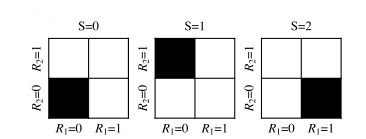
\includegraphics[height=4cm]{tex/example.jpg}
\caption{Probability distributions for $S\in\{0,1,2\}$ and$R_1,R_2\in\{0,1\}$.}
\label{fig8}
 
\end{figure}

\paragraph{Four Variables}
Now we consider a more complicated system with four variables, and we want to calculate the value of $\Pi_{\mathrm{R}}(S ; \{2\},\{13\})$.

On one hand, we can apply Equation \ref{ee1}  to solve the problem:
\begin{equation}\Pi_{\mathbf{R}}(S ;\{2\},\{13\})=I_{\min }(S ; \{2\},\{13\})-\sum_{s} p(s) \max _{\beta \in \alpha^{-}} \min _{\mathbf{B} \in \beta} I(S=s ; \mathbf{B})\label{43}\end{equation} 
where $\beta \in\{\{\{1\}\{2\}\},\{\{2\}\{3\}\}\} $ . Then we just need to expand the formula to get the result. 

On the other hand, based on the observations in Figure\ref{fig:pidiagram}(b), we can express the field using Equation \ref{eqn:intersectofbasic}:


\begin{equation}
    \begin{aligned}
    &\mu^{*}\left( \left\{ \tilde{R}_1 \right\}^{C} \cap \left\{ \tilde{R}_2 \right\}\cap \left\{ \tilde{R}_3 \right\}^{C} \cap \left\{\tilde{R}_{12} \right\}\cap \left\{\tilde{R}_{13} \right\}\cap \left\{\tilde{R}_{23} \right\}\cap \left\{\tilde{R}_{123} \right\} \right)  \\
   =&\mu^{*}\left(\left\{\tilde{R}_2 \right\}\cap  \left\{  \tilde{R}_{12} \right \}\cap  \left\{  \tilde{R}_{13} \right \} \cap  \left\{  \tilde{R}_{23} \right \}\cap \left\{\tilde{R}_{123} \right\}\right)  -\mu^{*}\left(\left\{\tilde{R}_1 \right\}\cap \left\{ \tilde{R}_2 \right\}\cap  \left\{  \tilde{R}_{12} \right \}\cap  \left\{  \tilde{R}_{13} \right \}\cap  \left\{  \tilde{R}_{23} \right \}\cap \left\{\tilde{R}_{123} \right\}\right)\\
    &-\mu^{*}\left(\left\{\tilde{R}_2 \right\}\cap \left\{ \tilde{R}_3 \right\}\cap  \left\{  \tilde{R}_{12} \right \}\cap  \left\{  \tilde{R}_{13} \right \} \cap  \left\{  \tilde{R}_{23} \right \}\cap \left\{\tilde{R}_{123} \right\}\right) \\
    &+\mu^{*}\left( \left\{ \tilde{R}_1 \right\} \cap \left\{ \tilde{R}_2 \right\}\cap \left\{ \tilde{R}_3 \right\} \cap \left\{\tilde{R}_{12} \right\}\cap \left\{\tilde{R}_{13} \right\}\cap \left\{\tilde{R}_{23} \right\}\cap \left\{\tilde{R}_{123} \right\} \right)\\
    =&I_{\min} \left( S; \left\{ 2 \right\} ,\left\{ 1, 2 \right\} ,\left\{ 1, 3 \right\},\left\{ 2, 3 \right\},\left\{ 1, 2, 3 \right\}\right)  - I_{\min} \left( S; \left\{ 1 \right\} ,\left\{ 2 \right\} ,\left\{ 1, 2 \right\} ,\left\{ 1, 3 \right\},\left\{ 2, 3 \right\},\left\{ 1, 2, 3 \right\}\right) \\
    &- I_{\min} \left( S; \left\{ 2 \right\} ,\left\{ 3 \right\} ,\left\{ 1, 2 \right\} ,\left\{ 1, 3 \right\},\left\{ 2, 3 \right\},\left\{ 1, 2, 3 \right\}\right) +I_{\min} \left( S; \left\{ 1 \right\} ,\left\{ 2 \right\} ,\left\{ 3 \right\} ,\left\{ 1, 2 \right\} ,\left\{ 1, 3 \right\},\left\{ 2, 3 \right\},\left\{ 1, 2, 3 \right\}\right)\\
    =&I_{\min} \left( S; \left\{ 2 \right\} ,\left\{ 1, 3 \right\}\right)  - I_{\min} \left( S; \left\{ 1 \right\} ,\left\{ 2 \right\} \right) - I_{\min} \left( S; \left\{ 2 \right\} ,\left\{ 3 \right\} \right) +I_{\min} \left( S; \left\{ 1 \right\} ,\left\{ 2 \right\} ,\left\{ 3 \right\} \right)
    \end{aligned}
\end{equation}


By some set operations, it can be translated into the linear combination of $I_{\min}$. The last equality holds because the former can be greatly simplified. For example, $\left\{ \tilde{R}_2 \right\} \subseteq \left\{\tilde{R}_1, \tilde{R}_2 \right\},\left\{\tilde{R}_2, \tilde{R}_3 \right\}\cdots$Now we just need to calculate the value of each $I_{min}$.\\

% What's more, we can also get the result applying Equation \ref{def:partial}, by which we can express $\Pi_{\mathbf{R}}$ using the linear combination of $I_{\min}$.\\

% We can list all $I_{\min}$ of the  sets which have the partial order relation with $\{\{2\},\{13\}\}$:

% \begin{equation}I_{\min }(S;\left\{2\},\{13\}\right)=\Pi_{\mathbf{R}}(S ;\{2\},\{3\})+\Pi_{\mathbf{R}}(S ;\{1\},\{2\})+\Pi_{\mathbf{R}}(S ;\{2\},\{13\})+I_{\min }(S;\left\{1\},\{2\},\{3\}\right)\label{44}\end{equation}

% \begin{equation}I_{\min }(S;\left\{2\},\{3\}\right)=\Pi_{\mathbf{R}}(S ;\{2\},\{3\})+I_{\min }(S;\left\{1\},\{2\},\{3\}\right)\label{45}\end{equation}

% \begin{equation}I_{\min }(S;\left\{1\},\{2\}\right)=\Pi_{\mathbf{R}}(S ;\{1\},\{2\})+I_{\min }(S;\left\{1\},\{2\},\{3\}\right)\label{46}\end{equation}

% Combine Equation \ref{44},\ref{45},\ref{46}, then we have the save result as before.\\

Now we use another simple example to illustrate the equivalence between the two expressions. Based on the probability distribution in Figure \ref{fig8}, we introduce another variable $R_3$. Consider the equally-probable cases of S as follows:
\[
\begin{array}{c}
S=0 \iff {R}_1=0,{R}_2=0,{R}_3=0\\
S=1 \iff {R}_1=0,{R}_2=1,{R}_3=1\\
S=2 \iff {R}_1=1,{R}_2=0,{R}_3=0\\
\end{array}
\]

On one hand, by applying Equation \ref{43}, we have
\begin{equation}I_{\min }(S ; \{2\},\{13\})=\log3 -\frac{2}{3} \log 2\end{equation}
\begin{equation}\sum_{s} p(s) \max _{\beta \in \alpha^{-}} \min _{\mathbf{B} \in \beta} I(S=s ; \mathbf{B})=\log3 -\frac{2}{3} \log 2\end{equation}
So $\Pi_{\mathrm{R}}(S ; \{2\},\{13\})$=0.\\

On the other hand, by calculating by the linear combination of $I_{\min}$, we can also have the same outcome. In other words,
\begin{equation}I_{\min} \left( S; \left\{ 1 \right\} ,\left\{ 2 \right\} \right) - I_{\min} \left( S; \left\{ 2 \right\} ,\left\{ 3 \right\} \right) +I_{\min} \left( S; \left\{ 1 \right\} ,\left\{ 2 \right\} ,\left\{ 3 \right\}\right)=\sum_{s} p(s) \max _{\beta \in \alpha^{-}} \min _{\mathbf{B} \in \beta} I(S=s ; \mathbf{B})\end{equation}


